\section{Defintions}



\begin{comment}
\cite{} establishes that driving at a constant speed is more fuel echonomic. 
From observing the data with and without the driver using cruise control we find that the speed varies $\pm$ 1km/h. 
An experienced driver can drive at a constant speed without cruise control but the speed will generaly vary more. 
We define a vehicle as cruising if it in a 40 second period drive with a constant speed $\pm$ 1km/h.

Figure~\ref{fig:cruiseTrips} shows how often the trips cruise. 
Almost all trips never cruise, and all trips classified as having a low km/l never cruise.

\end{comment}

\subsection{Acceleration kilometers}
Acckm$_t$ is the total km driven while accelerating for a given trip $t$, normalised by the lenght of the trip. 
It is established in \cite{EcoMark} that accelerrating consume extra fuel and a trip with a few acceleration kilometers should therefore use less fuel.  
Acckm is caculated as in Algorithm \ref{alg.acckm}. 
A buffer (dotted line) as shown in Figure \ref{fig:acckm} is implemented to prevent small speed variations (solid line) in effecting acckm.

\begin{algorithm}
\caption{$acckm$}\label{alg.acckm}
\begin{algorithmic}[1]
\State $temp = 0$
\State $counter = 0$
\State $buffer = 1$ %TODO: Changed to 1. Do this in code.
\While{$i < n$}
\If{$v_i - v_{i-1} > buffer$}
	\State $counter += (v_i - v_{i-1}) - buffer$
	\State $temp = v_i - buffer$
\ElsIf{$v_{i-1} - v_i > buffer$}
	\State $temp = v_i + buffer$
\EndIf
\State $i+=1$
\EndWhile
\State \Return $ counter / trip_{length}$

\end{algorithmic}
\end{algorithm}

Figure \ref{fig:acckm} shows the number of trips on the y-axis having a acckm show on the x-axis. 
Trips with a high km/l are mostly clustered with a low acckm and a trips in the \fuelMedium class . 

\begin{figure}[htb]
\centering
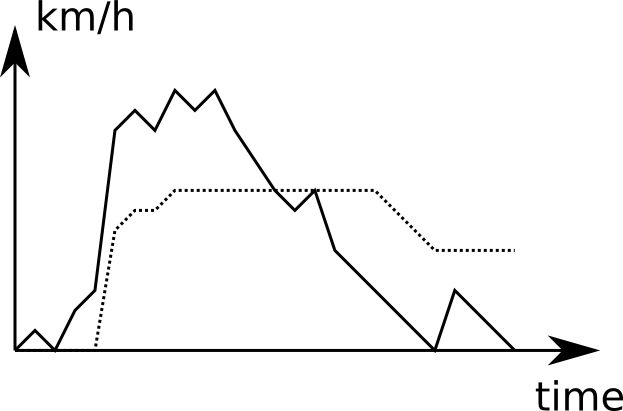
\includegraphics[width=0.4\textwidth]{../images/acckm.png}
\caption{Acckm}
\label{fig:acckm}
\end{figure}

\begin{figure}
\centering
\includegraphics[width=0.45\textwidth]{../src/images/acckmTrips.png}
\caption{Acceleration kilometers}
\label{fig:acckmTrips}
\end{figure}

\subsection{Stop and go}
Stop and go behaviour is not fuel efficient as more fuel is consumed when accelerating than when driving at a constant speed.
It is therefore interesting to see if the number of times a vehicle stops and drives on is correlated with km/l.
We say a vehicle is stopped when it decelerations below 10 km/h and that it drives again when it accelerates up above 15 km/h.
TODO: Explain why.

%TODO: Experiments

Figure~\ref{fig:stopngoTrips} shows the number of stop-and-goes of each trip normalised with the length of that trip versus the km/l of the trip.
The size of the plot indicates the amount of fuel used in the trip and the color signals what class it has been asigned to.
We see that the trips in the \fuelHigh class have few stop and goes and about half of the trips in the \fuelMedium class have more stop and goes.

\begin{figure}
\centering
\includegraphics[width=0.45\textwidth]{../src/images/stopngoTrips.png}
\caption{Number of stop and goes}
\label{fig:stopngoTrips}
\end{figure}
